% mnras_template.tex
%
% LaTeX template for creating an MNRAS paper
%
% v3.0 released 14 May 2015
% (version numbers match those of mnras.cls)
%
% Copyright (C) Royal Astronomical Society 2015
% Authors:
% Keith T. Smith (Royal Astronomical Society)

% Change log
%
% v3.0 May 2015
%    Renamed to match the new package name
%    Version number matches mnras.cls
%    A few minor tweaks to wording
% v1.0 September 2013
%    Beta testing only - never publicly released
%    First version: a simple (ish) template for creating an MNRAS paper

%%%%%%%%%%%%%%%%%%%%%%%%%%%%%%%%%%%%%%%%%%%%%%%%%%
% Basic setup. Most papers should leave these options alone.
\documentclass[a4paper,fleqn,usenatbib]{mnras}

% MNRAS is set in Times font. If you don't have this installed (most LaTeX
% installations will be fine) or prefer the old Computer Modern fonts, comment
% out the following line
\usepackage{newtxtext,newtxmath}
% Depending on your LaTeX fonts installation, you might get better results with one of these:
%\usepackage{mathptmx}
%\usepackage{txfonts}

% Use vector fonts, so it zooms properly in on-screen viewing software
% Don't change these lines unless you know what you are doing
\usepackage[T1]{fontenc}
\usepackage{ae,aecompl}


%%%%% AUTHORS - PLACE YOUR OWN PACKAGES HERE %%%%%
% \usepackage(graphicx,tabularx}

% Only include extra packages if you really need them. Common packages are:
\usepackage{graphicx}	% Including figure files
\usepackage{amsmath}	% Advanced maths commands
\usepackage{amssymb}	% Extra maths symbols

%%%%%%%%%%%%%%%%%%%%%%%%%%%%%%%%%%%%%%%%%%%%%%%%%%

%%%%% AUTHORS - PLACE YOUR OWN COMMANDS HERE %%%%%

% Please keep new commands to a minimum, and use \newcommand not \def to avoid
% overwriting existing commands. Example:
%\newcommand{\pcm}{\,cm$^{-2}$}	% per cm-squared

%%%%%%%%%%%%%%%%%%%%%%%%%%%%%%%%%%%%%%%%%%%%%%%%%%

%%%%%%%%%%%%%%%%%%% TITLE PAGE %%%%%%%%%%%%%%%%%%%

% Title of the paper, and the short title which is used in the headers.
% Keep the title short and informative.
\title[CRTS\,J0711+4404]{CRTS\,J0711+4404: Time resolved spectra and high speed photometry of an eclipsing polar}

% The list of authors, and the short list which is used in the headers.
% If you need two or more lines of authors, add an extra line using \newauthor
\author[R.P. Ashley et al.]{
R.P. Ashley$^{1}$\thanks{E-mail: r.p.ashley@warwick.ac.uk},
A. Aungwerojwit$^{2, 3}$,
B.T. G{\"a}nsicke$^{1}$,
M.A. Hollands$^{1}$,
T.R. Marsh$^{1}$ and \newauthor
John Southworth$^{4}$
\\
% List of institutions
$^{1}$Department of Physics, University of Warwick, Gibbet Hill Road, Coventry, CV4 7AL, UK\\
$^{2}$Department of Physics, Faculty of Science, Naresuan University, Phitsanulok 65000, Thailand\\
$^{3}$ThEP Center, CHE, 328 Si Ayutthaya Road, Bangkok 10400, Thailand\\
$^{4}$Astrophysics Group, Keele University, Staffordshire, ST5 5BG, UK
}

% These dates will be filled out by the publisher
\date{Accepted XXX. Received YYY; in original form ZZZ}

% Enter the current year, for the copyright statements etc.
\pubyear{2015}

% Don't change these lines
\begin{document}
\label{firstpage}
\pagerange{\pageref{firstpage}--\pageref{lastpage}}
\maketitle

% Abstract of the paper
\begin{abstract}
CSS081231:071126+440405 is an eclipsing polar with a period of 117 minutes. Small and medium sized telescopes have photometry of the system dating back to late 2008. The ephemeris was computed shortly after discovery and then revised recently following five years of subsequent observations. Newer photometric observations have allowed us to place tighter contraints on the orbital parameters. We have obtained six optical spectra of the system covering phases 0.24 to 0.90 during outburst and sixteen optical spectra taken during quiescence including a spectrum taken during the primary eclipse revealing the spectral type of the donor star to be dM5.5. The spectra show clear cyclotron humps modulating during the orbital cycle. The surface magnetic field strength at the accreting pole is $B  \sim 34 MG$.
\end{abstract}

% Select between one and six entries from the list of approved keywords.
% Don't make up new ones.
\begin{keywords}
stars -- individual -- CSS081231:071126+440405 -- binares: eclipsing -- stars: cataclysmic variables
\end{keywords}

%%%%%%%%%%%%%%%%%%%%%%%%%%%%%%%%%%%%%%%%%%%%%%%%%%

%%%%%%%%%%%%%%%%% BODY OF PAPER %%%%%%%%%%%%%%%%%%

\section{Introduction}
CSS081231:071126+440405 (hereafter,  CRTS\,J0711+4404) is an eclipsing polar cataclysmic variable..... more intro ....

\section{Observations}
\subsection{High speed photometry}

Six nights of photometry were obtained using ULTRASPEC \citep{ULTRASPEC}, mounted on the 2.5m Thai National Telescope during 2014 and 2015. Exposure times varied from 1.6 to 3.6 seconds depending on the conditions of the night. For the first three observations the Sloane g filter was used and for the last three observations the KG5 filter was used. The KG5 filter has a broad optical passband stretching from $\sim3500 \AA~ \mbox{to} \sim7000 \AA$ and was chosen to allow the maximum light throughput while avoiding contamination from the M dwarf companion.  Data was reduced using the ULTRACAM reduction pipeline (Marsh reference) with a comparison star located about 35 arcseconds to the W from the target and located at RA 07:11:23, DEC +44:04:13 (J2000). The details for these nights are shown in Table \ref{tab:photometry}. 

\begin{table}
  \caption{Photometry used in this study. The instrument used was ULTRASPEC, mounted on the 2.5m Thai National Telescope at the Thai National Observatory.}
  \begin{tabular}{ l  l  l  l  l  }
  \hline
  Date & BJD & Filter & $T_{\mbox{exp}}(s)$& Total time (min)\\
  \hline
    2014/02/06 & 2456695 & Sloan g & 1.6 & 147.8 \\
    2014/02/07 & 2456696 & Sloan g & 1.7 & 166.2 \\
    2014/02/08 & 2456697 & Sloan g & 2.8 & 73.6 \\
    2014/12/12 & 2457004 & KG5 & 3.6 & 95.1 \\
    2015/01/01 & 2457024 & KG5 & 2.0 & 118.2 \\
    2015/01/03 & 2457026 & KG5 & 2.0 & 131.1 \\
    
  \hline
  \end{tabular}
  \label{tab:photometry}
\end{table}

As in previous observations, the light curves display strong flickering variability and a steep-sided eclipse. \citet{Schwope2015} finds pre-eclipse dips at phase xx. We do not see the equivalent dips in any of our seven light curves. It is possible, as discussed by Schwope that the cause of these dips, namely, the self-occultation of the accretion stream is a transient feature and was not present on during our observations. \emph{If there are any differences between the g-band and the KG5 light curves, mention and explain.}

\subsection{Phase resolved spectroscopy}
CRTS\,J0711+4404 was observed on two separate nights. Once in February 2009 when it was in quiescence and then again in December 2014 during outburst. On both nights the target was observed using the ISIS dual-beam spectrograph on the William Herschel Telescope in La Palma. During the 2009 observations, 17 spectra were taken in the optical region, spanning a wavelength range of  $4200$\AA\, to $8800$\AA\, with a typical dispersion of $0.23-0.93$\AA\, per pixel. The spectra covered all phases of an orbit. The gratings used were the R1200 in the blue arm and the R316R in the red arm. In December 2014, six spectra were obtained covering a wavelength range of $\lambda\lambda 3200 \AA$ to $9200 \AA$ with a typical dispersion of $0.86 - 1.81 \AA$ per pixel. In both cases pixels were binned to factor of 2 in the dispersion direction. 

\subsection{X-ray fluxes}
CRTS\,J0711+4404 is not a ROSAT source, but it appears in the Swift X-Ray Telescope Point Source Catalog \citep{2014ApJS..210....8E}. It was detected at $3.36 ^{+0.83} _{-0.72} cts/s$ in the full 0.3-10keV band, but the fluxes for the individual soft, medium and hard bands are also given. It is available from Vizier as catalogue IX/43.
\emph{Comment: Need to include a longer discussion of the newer Schwope paper here... or leave out this section altogether.}

\section{Analysis}

\subsection{Eclipse timings}
The primary eclipse was observed 7 times on 6 different nights.  We converted all eclipse times to barycentric dynamical time (TDB) in the form of modified Julian days and corrected to the barycentre of the Solar System, giving what we refer to as BMJD(TDB).

For all our new data we determined the time of mid-egress by a least-squares fit of a function composed of a sigmoid and a straight line of the form, 
\begin{equation}f = \frac{a_1}{1+e^{-a_2(x-a_3)}} + a_4 + a_5(x - a_3)\end{equation}
where $f$ and $x$ are the flux measurements and timing of our observations and $a_1$ to $a_5$ are the fit parameters with $a_3$ being the time at which ingress or egress occurs. 

In order to measure the centre of the eclipse, we fitted this function to both the ingress and the egress for each eclipse and then used the mid-point between these two values as our eclipse time. Using this method we measure the eclipse ingress and egress times to a typical precision of 0.3 seconds. All eclipse timings are reported in Table \ref{tab:eclipses}. Light-curves of all of the eclipses are shown in Fig. \ref{fig:stacked-eclipses}. 

\begin{table}
  \caption{Details of the 7 primary eclipses. Ingress, egress and centre of eclipse times are shown as time since start of BJD (days).}
  \begin{tabular}{ l  l  l  l  l  }
  \hline
 	BJD & Ingress & Egress & Centre & Duration (s) \\
  \hline
    2456695 & 0.269480 & 0.274504 & 0.2719921 & 434.1(0.3) \\
    2456696 & 0.245999 & 0.251026 & 0.2485129 & 434.4(0.2) \\
    2456696 & 0.327374 & 0.332403 & 0.3298889 & 434.5(0.1) \\
    2456697 & 0.222525 & 0.227548 & 0.2250372 & 434.0(0.2) \\
    2457004 & 0.338635 & 0.343661 & 0.3411487 & 434.3(0.2) \\
    2457024 & 0.357335 & 0.362353 & 0.3598445 & 433.6(0.3) \\
    2457026 & 0.310374 & 0.315401 & 0.3128882 & 434.3(0.3) \\
  \hline
  \end{tabular}
  \label{tab:eclipses}
\end{table}

Small and medium sized telescopes have photometry of the system dating back to late 2008. These observations were compiled and reported by \citet{Schwope2015}. Schwope revised the original ephemeris that was published shortly by  \citet{Thorne2010}. The ephemeris given by Schwope is 
\begin{equation}BJD(TDB) = 2454833.207868(14) + E\times0.0813768094(6)\end{equation}
but since our observations have been taken with instruments operating at a much higher time resolution than the sources used by Schwope, we have re-computed the ephemeris by combining our own eclipse times with those documented in the Schwope paper. Our recomputed ephemeris is 
\begin{equation}BJD(TDB) = 2454833.207854(12) + E\times0.0813768096(5)\label{eq:ephemeris}\end{equation}
a revised O-C plot is shown in Fig. \ref{fig:ocdiagram} with the new eclipse times are indicated in green. The light curves for all of our high time resolution photometry is shown in Fig. \ref{fig:lightcurves}.

% O-C Diagram
\begin{figure}
	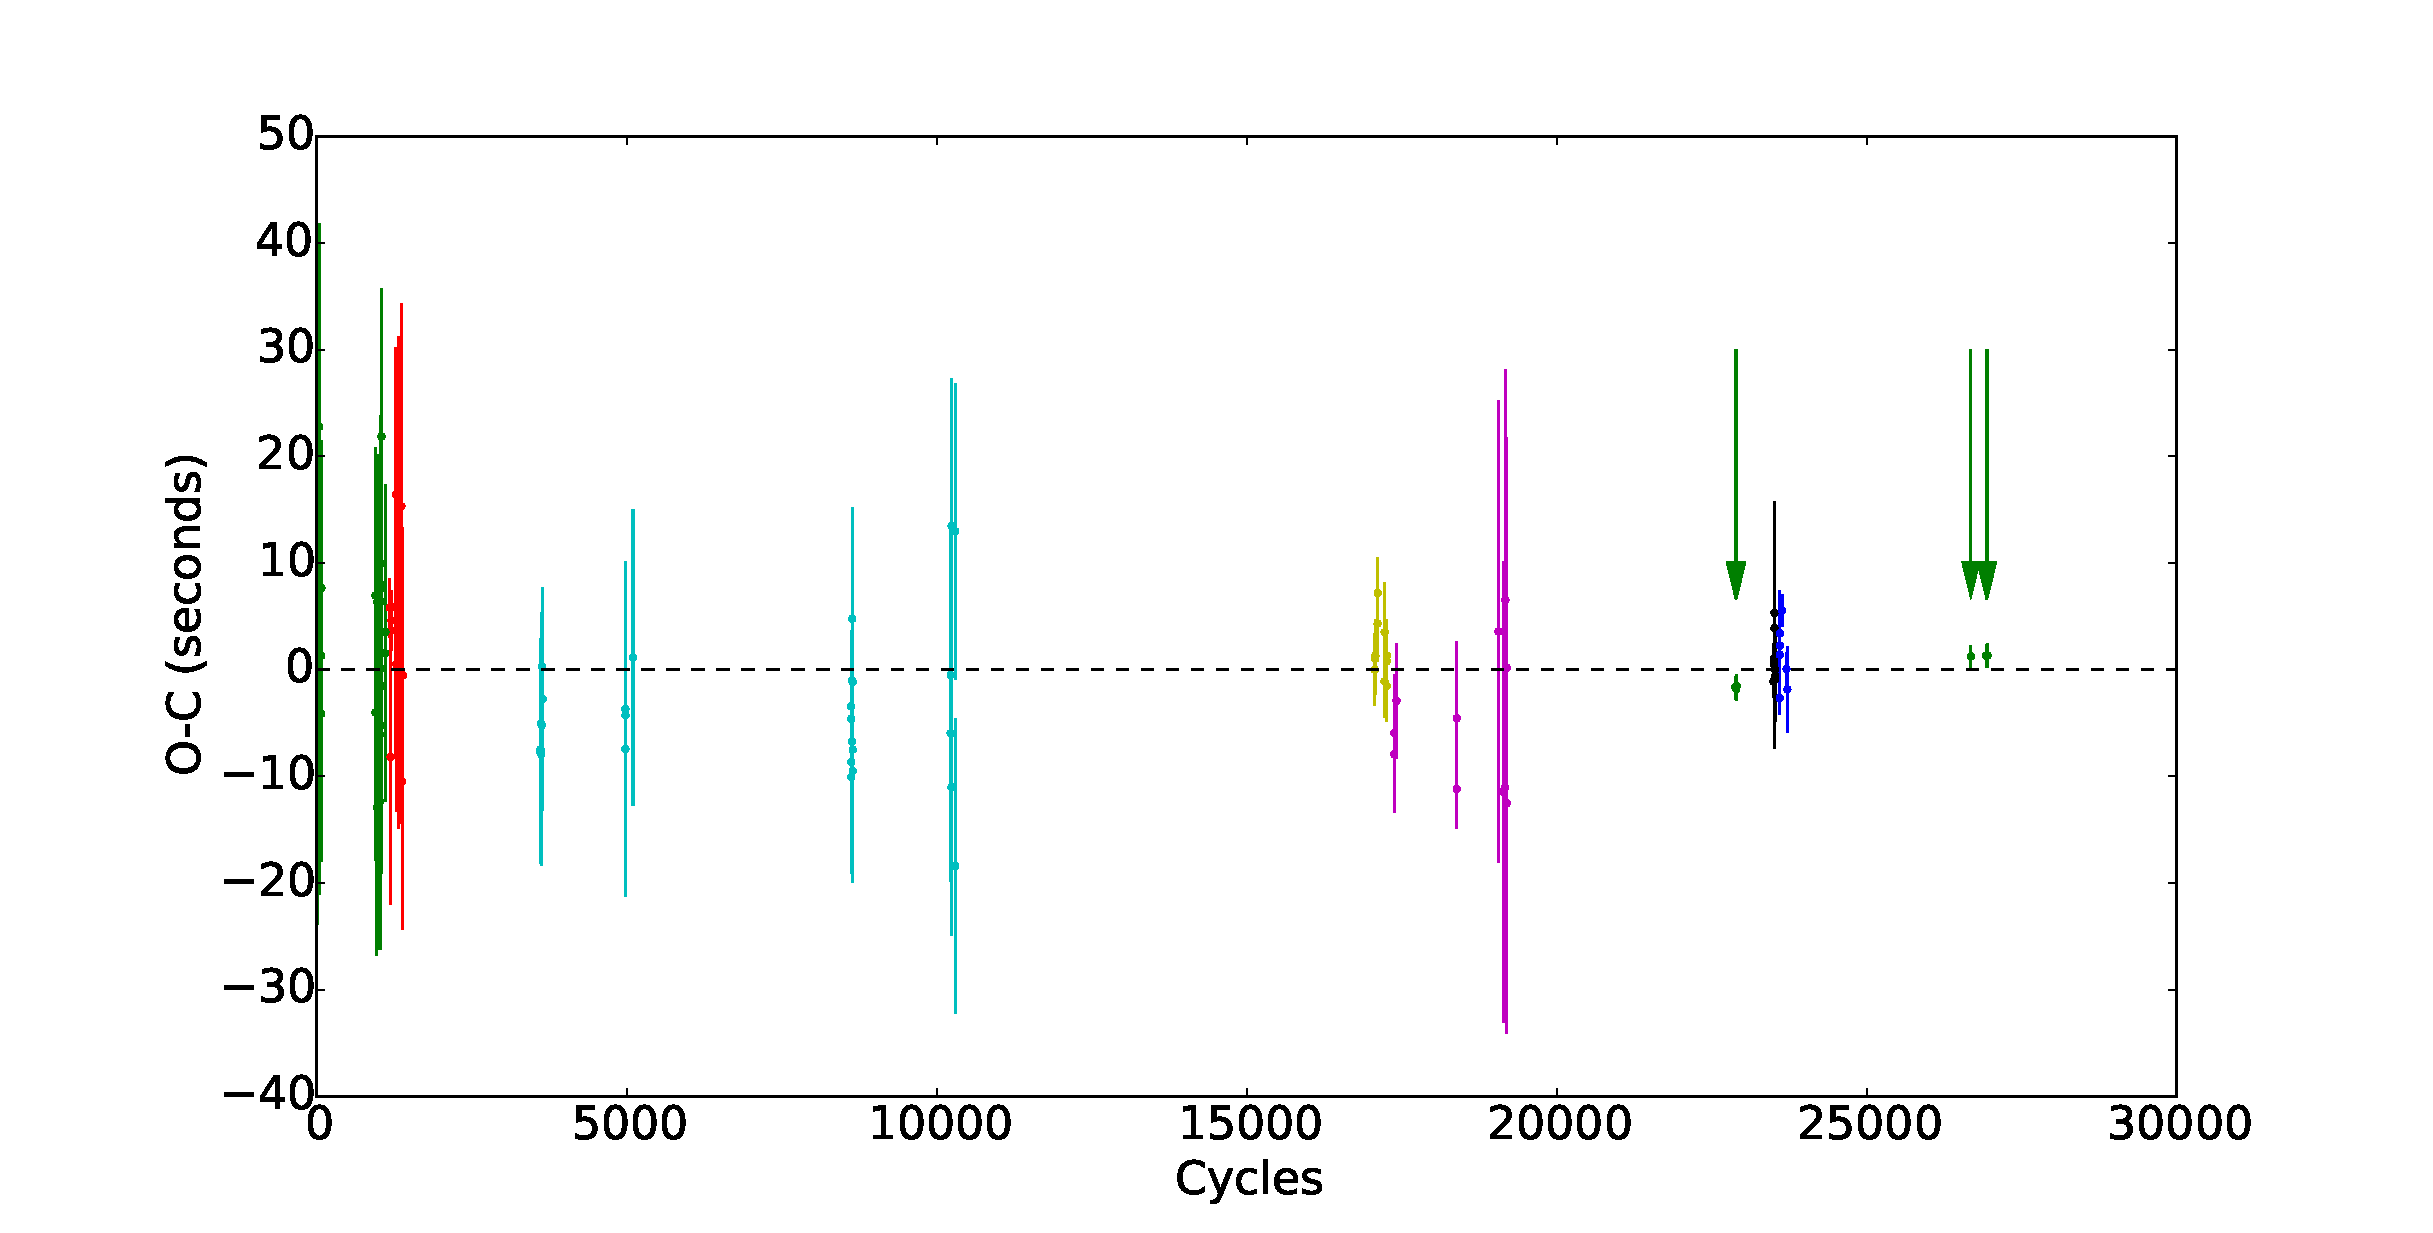
\includegraphics[width=\columnwidth]{images/css081231_oc.eps}
    \caption{The observed minus calculated times for all of the eclipse data as reported by \citet{Schwope2015} with our additional observations indicated by the green arrows in the diagram.  }
    \label{fig:ocdiagram}
\end{figure}

% TNT light curves.
\begin{figure*}
\centering
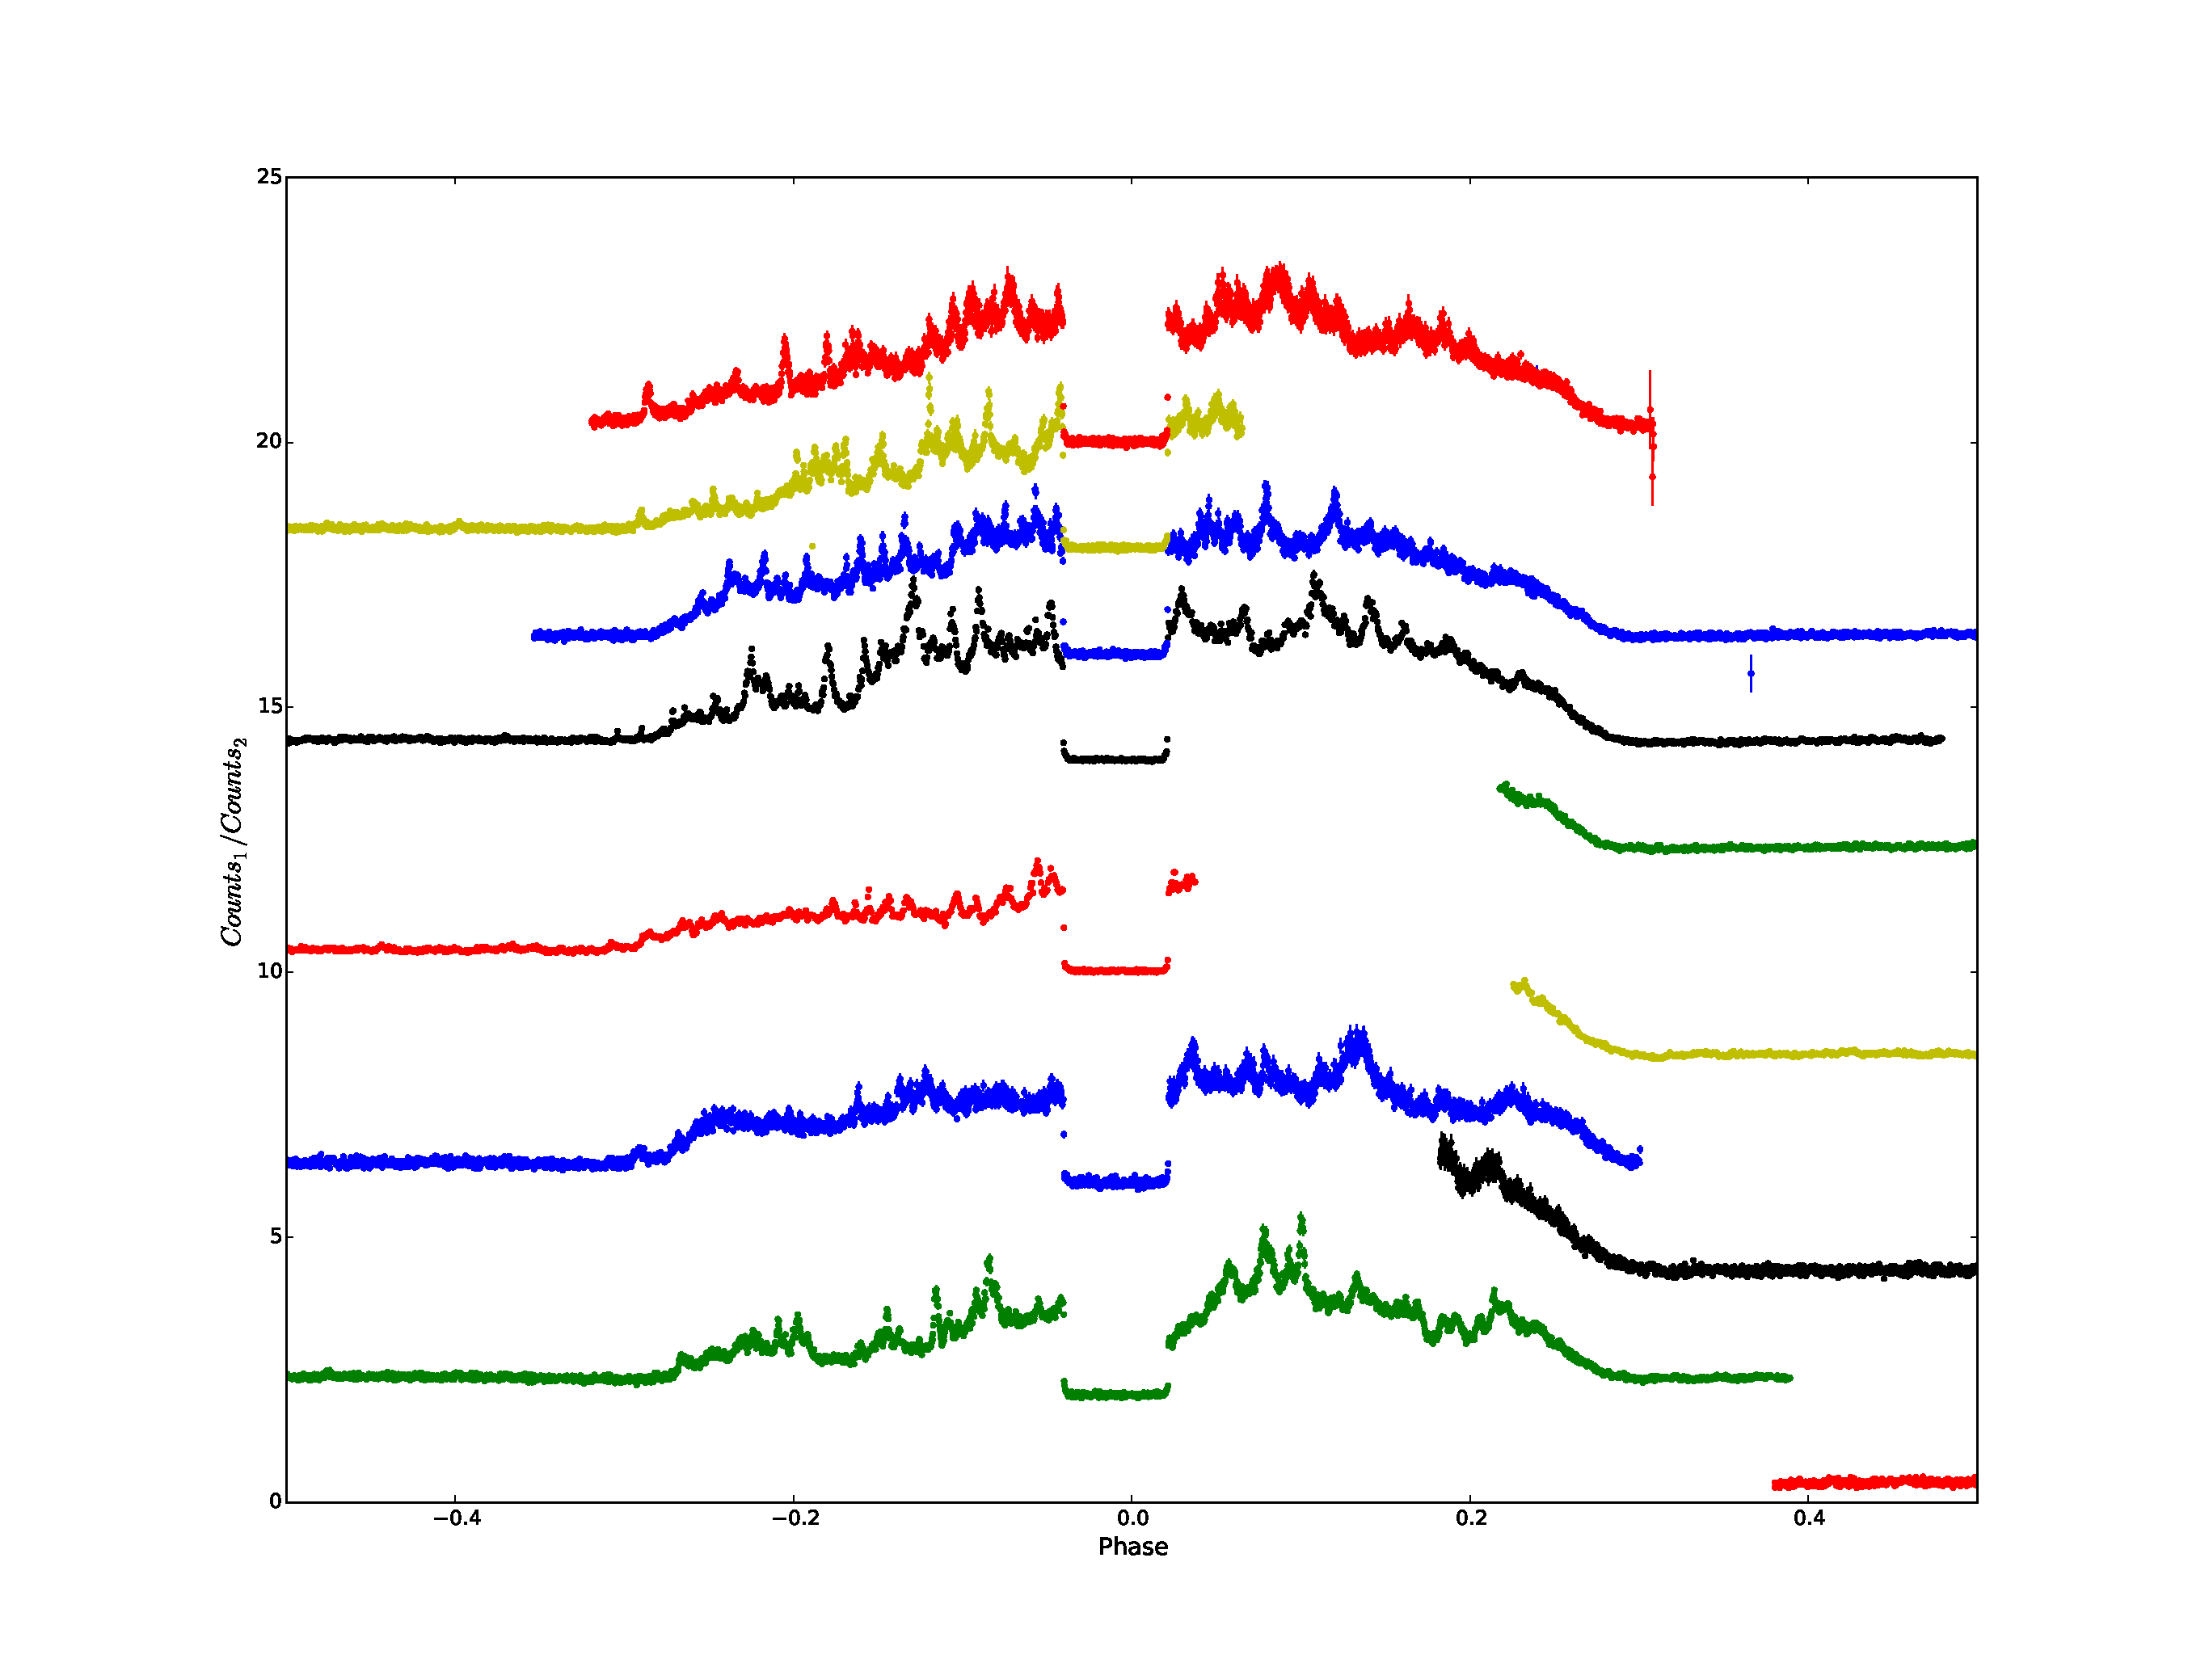
\includegraphics[width=\textwidth]{images/CSS081231_TNT_photometry.eps}
\caption[Caption for photometry]{ \emph{This figure to be removed. Only here for reference for the time being.}The light curves of CRTS\,J0711+4404. Exposure lengths vary from 1.6 to 3.6 seconds. The brightness of our target is measured as the fractional counts relative to our comparison star (described in the text). Each orbit is offset by 2 units for clarity.}
\label{fig:lightcurves}
\end{figure*}

% Stacked eclipses
\begin{figure}
\centering
\includegraphics[width=\columnwidth]{images/stacked_eclipses.eps}
\caption{The eclipse profiles of all seven of the eclipses recorded at the Thai National Telescope. The flux ratio is the counts for the target star compared to counts for our comparison (as described in the text). Each eclipse is shown with the MJD of the day it was taken. Two eclipses were observed on the night of 2014-02-07 (MJD 56695). Each light-curve is offset by 4 units for clarity.}
\label{fig:stacked-eclipses}
\end{figure}


% Example egress fit
\begin{figure}
\centering
\includegraphics[height=\columnwidth, angle=270]{images/egress.eps}
\caption[Caption for egress]{An example of the sigmoid fitting method applied to an egress of the primary eclipse. The vertical dashed line is the value used as the time measure of the eclipse egress.}
\label{fig:egress}
\end{figure}

\emph{Comment: Schwope states "Photometric observations with high time resolution during a low state would be most useful to directly measure the size of the white dwarf and high-speed photometric observations during a high state would allow to measure the size and location (azimuth) of the accretion spot directly."  Is there any more I can say/deduce about this?}

\subsection{Donor star spectral type}
In order to determine the spectral type of the M-dwarf, a spectrum taken during primary eclipse was matched to templates of M-dwarfs M0 to M9 taken from the SDSS catalog \citep{Bochanski2007}. Careful choice of the exposures ensured that we have a 300 second exposure taken entirely within the 433 second duration eclipse. The spectrum taken at phase 0.99 in Fig. \ref{fig:spectra-quiescent} is a 300s exposure centred on phase 0.99 and runs from phase 0.97 to 1.01.  Inspection of the eclipse profiles shown in Fig. \ref{fig:stacked-eclipses} shows that this spectrum covers only those phases that are in full eclipse and we can conclude that it is a spectrum of the M-dwarf only (ie without contamination from the White Dwarf or the accretion stream). We fitted this spectrum to a set  of template spectra taken from the SDSS catalog (reference) spanning spectral types dM0 to dM9. Our best fit spectrum is that of a dM5 and this is shown in Fig. \ref{fig:sloanfit}. 

\citet{WadeHorne1988} describe a method of determining the spectral type of the M dwarf companion using the relative strength of the TiO features. The idea is that, although equivalent widths of TiO features cannot be used directly since they are affected by the white dwarf and disc features (in our case, the dominant contaminant is the flux from the cyclotron radiation), the \emph{flux deficits} relative to a reference continuum are not affected. This method uses the following flux density measurements

\begin{equation}
	d_{\nu}(\lambda7165) = \frac{\int_{7140}^{7190}[c_\nu(\lambda)-f_\nu(\lambda)]d\lambda/\lambda}{\int_{7140}^{7190}d\lambda/\lambda}
\end{equation}
\begin{equation}
	d_{\nu}(\lambda7665) = \frac{\int_{7640}^{7690}[c_\nu(\lambda)-f_\nu(\lambda)]d\lambda/\lambda}{\int_{7640}^{7690}d\lambda/\lambda}
\end{equation}
where $c_\nu(\lambda)$ is derived by fitting a least-squares straight line to the observed flux $f_\nu(\lambda)$ in the continuum bands at ($7450-7550\AA$), ($8130-8170\AA$) and ($8222-8262\AA$).

The dimensionless parameters $\frac{d_{\nu}(\lambda7665)}{c_\nu(\lambda7665)}$ and $\frac{d_{\nu}(\lambda7665)}{d_{\nu}(\lambda7165)}$ were calculated for the spectrum taken at phase 0.99 (during the primary eclipse) as $0.4$ and $0.9$ respectively, placing the spectral type of the M dwarf as M5 according to table 3 in \citet{WadeHorne1988}.   

% Radial velocity fit
\begin{figure}
\centering
\includegraphics[height=\columnwidth, angle=270]{images/NaIrvfit.eps}
\caption[Caption for RVs]{A fit to the computed radial velocities of the Na I doublet at 8183\AA~ and 8194\AA. The $K_2$ amplitude for the fit is 435(12) km/s.  The period was fixed to 117 minutes as determined from the optical photometry and defined in equation \ref{eq:ephemeris}. }
\label{fig:rv-fit}
\end{figure}

% Outburst spectra
\begin{figure*}
\centering
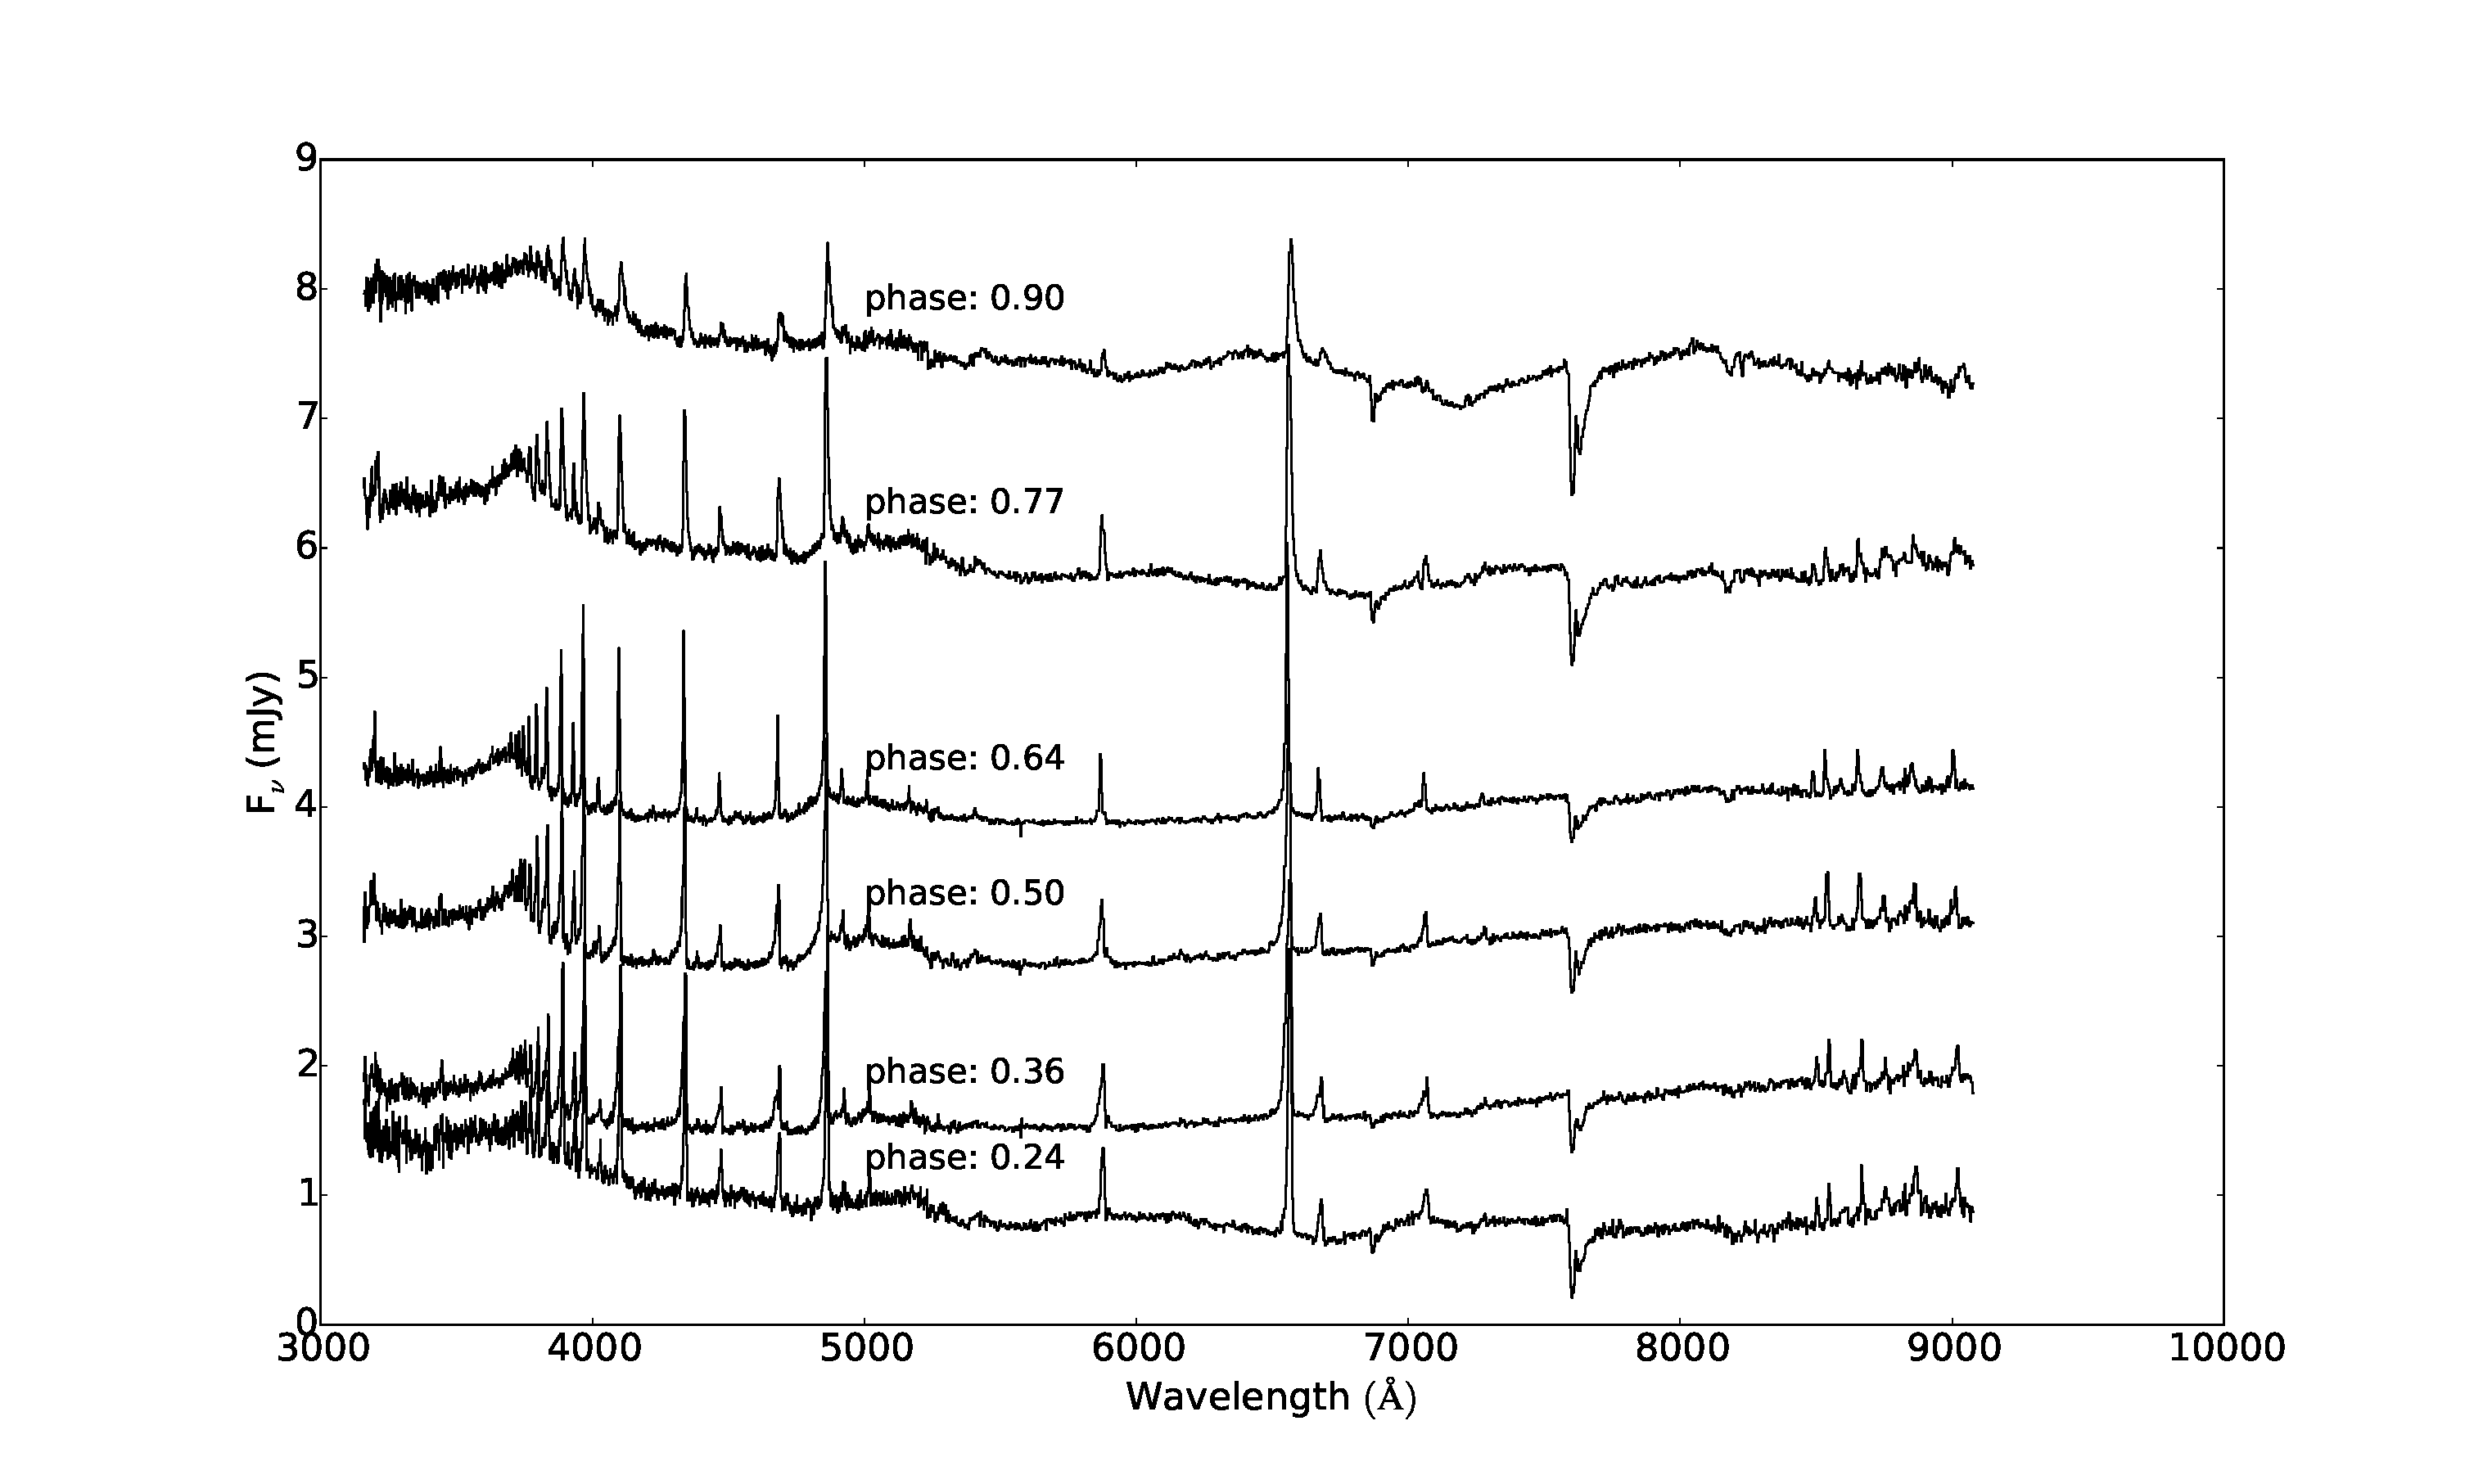
\includegraphics[width=\textwidth]{images/CSS081231_spectra.eps}
\caption[Caption for spectra]{The optical spectra of CSS081231 taken at 6 stages of the orbital cycle during outburst in December 2014. Cyclotron humps are seen in the early and late stages of the orbit when the accretion spot is in view. During the mid-phases of the orbit the accretion spot is eclipsed by the white dwarf. }
\label{fig:spectra-outburst}
\end{figure*}

% Quiescent spectra
\begin{figure*}
\centering
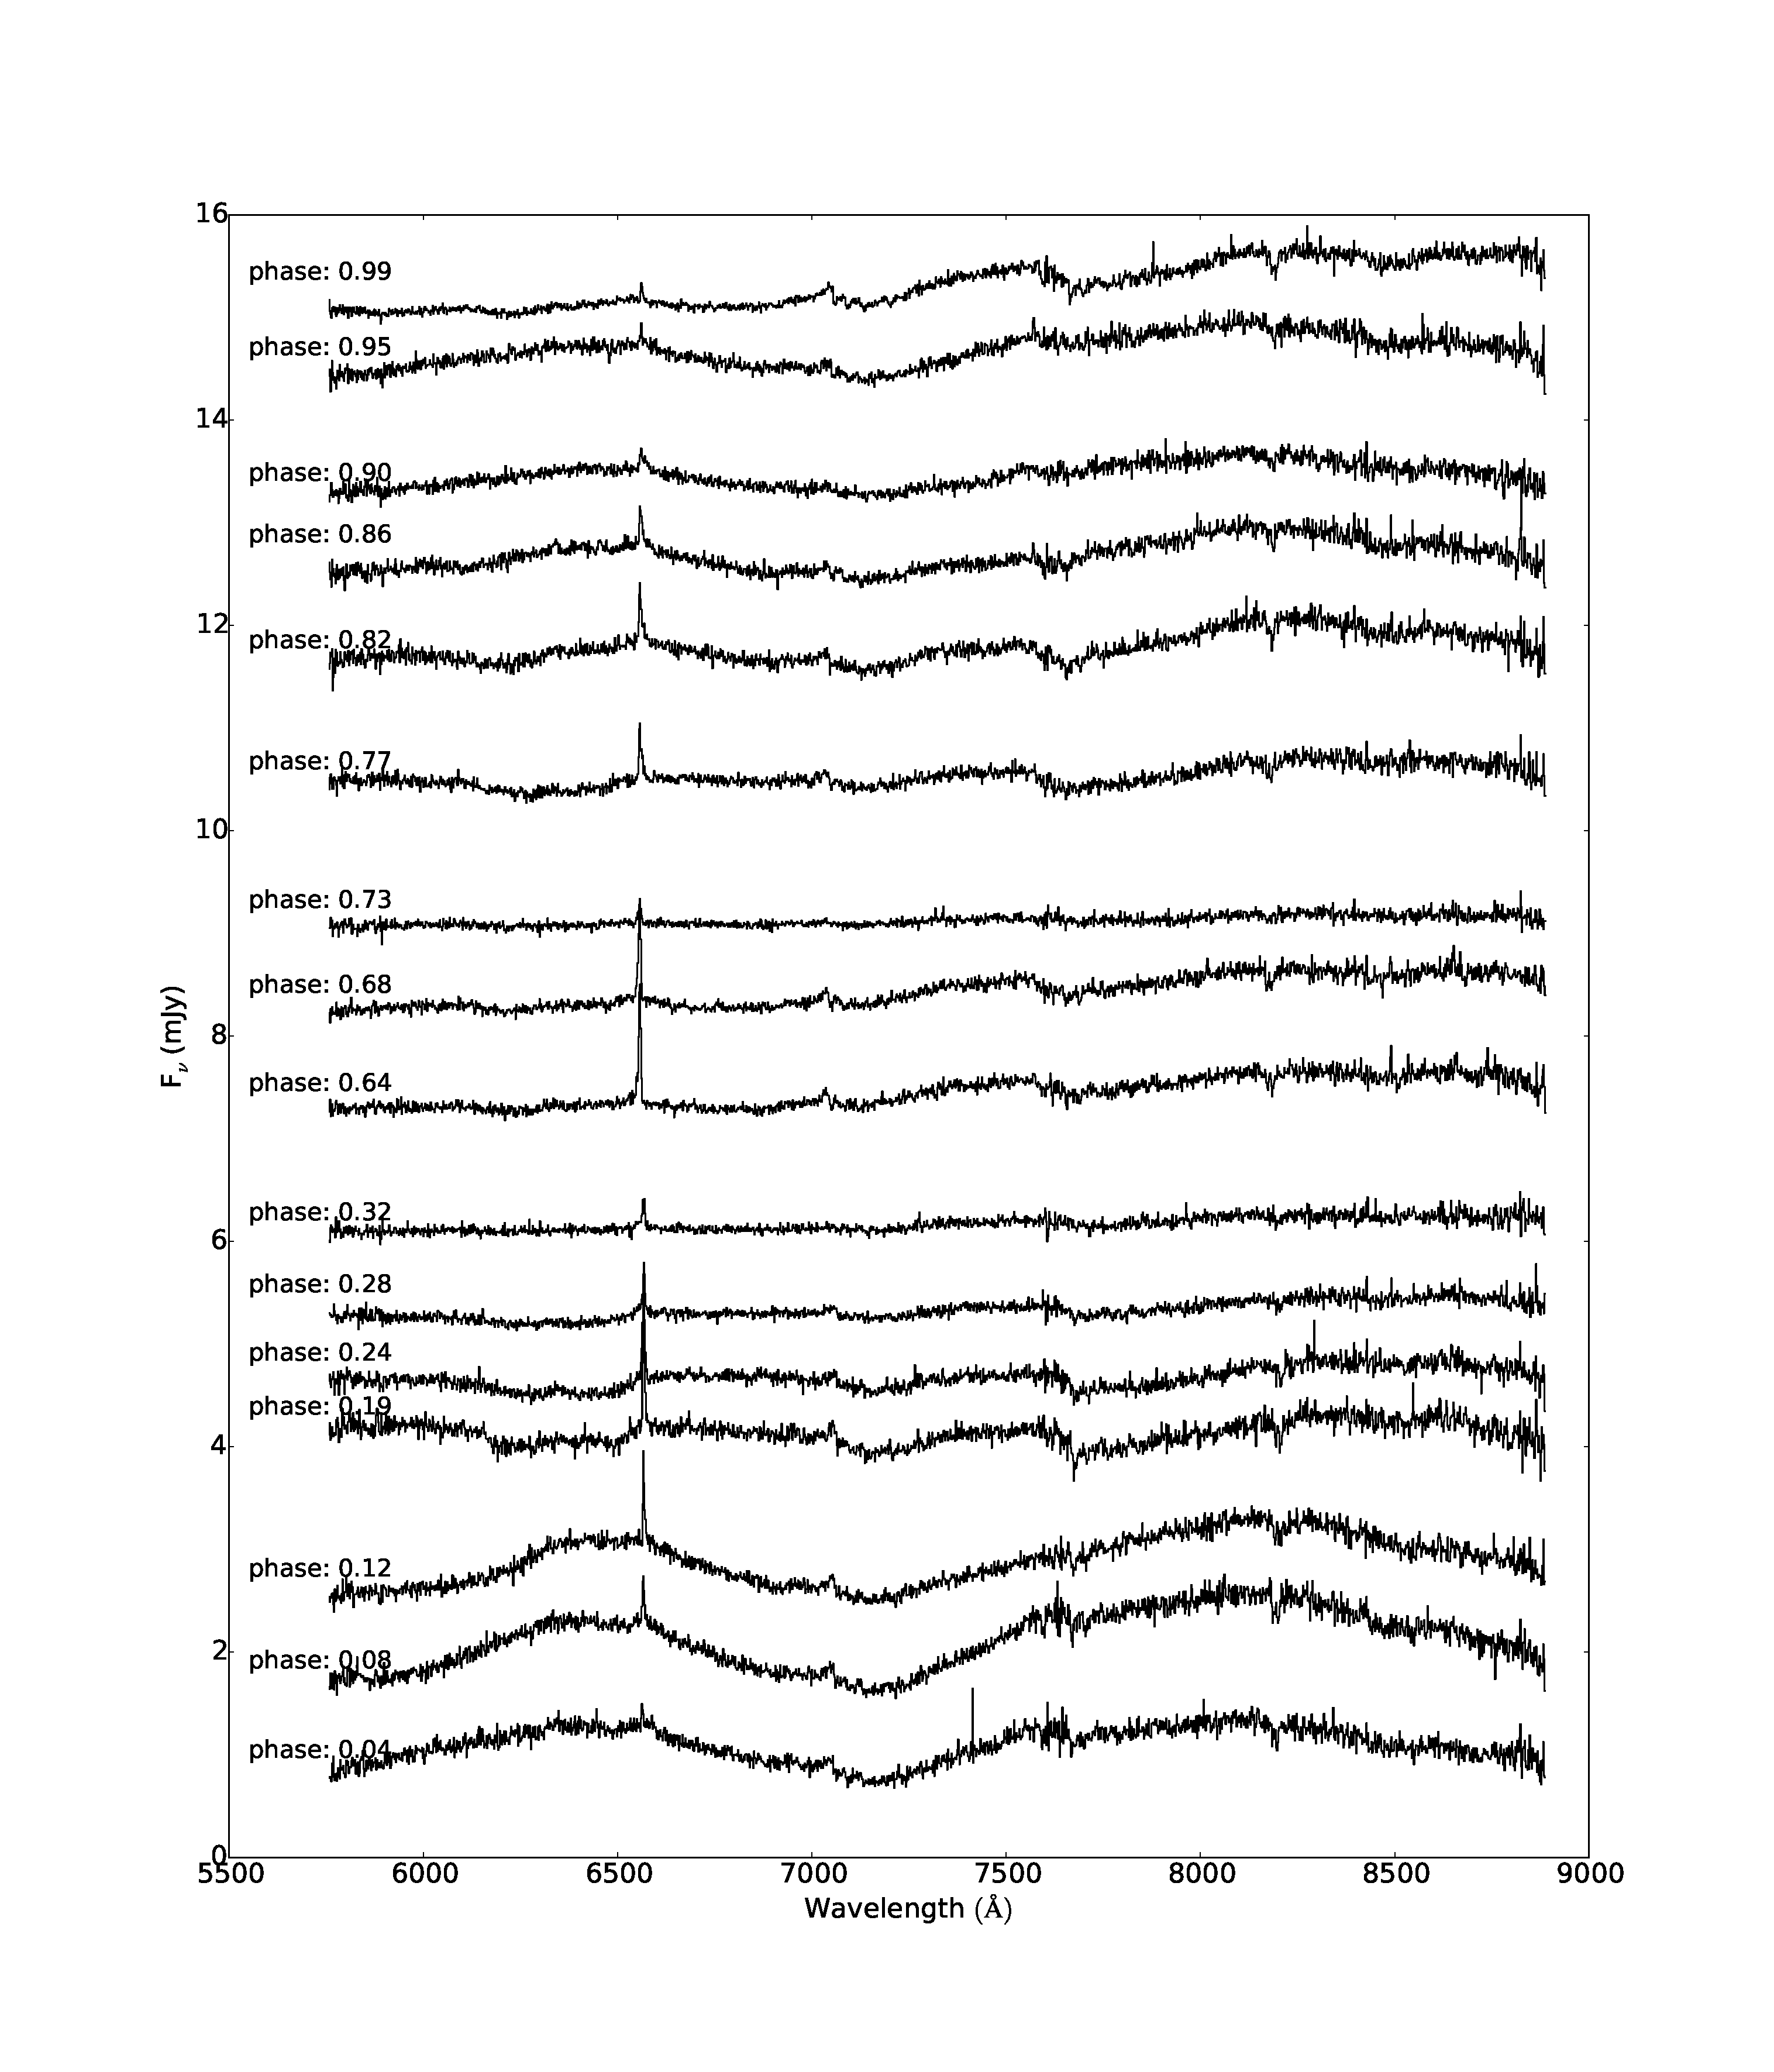
\includegraphics[width=\textwidth]{images/CSS081231_spectra_q.eps}
\caption[Caption for spectra]{The optical spectra of CRTS\,J0711+4404 taken at 16 stages of the orbital cycle during quiesence in February 2009.  }
\label{fig:spectra-quiescent}
\end{figure*}

% Quiescent spectra - blue
\begin{figure*}
\centering
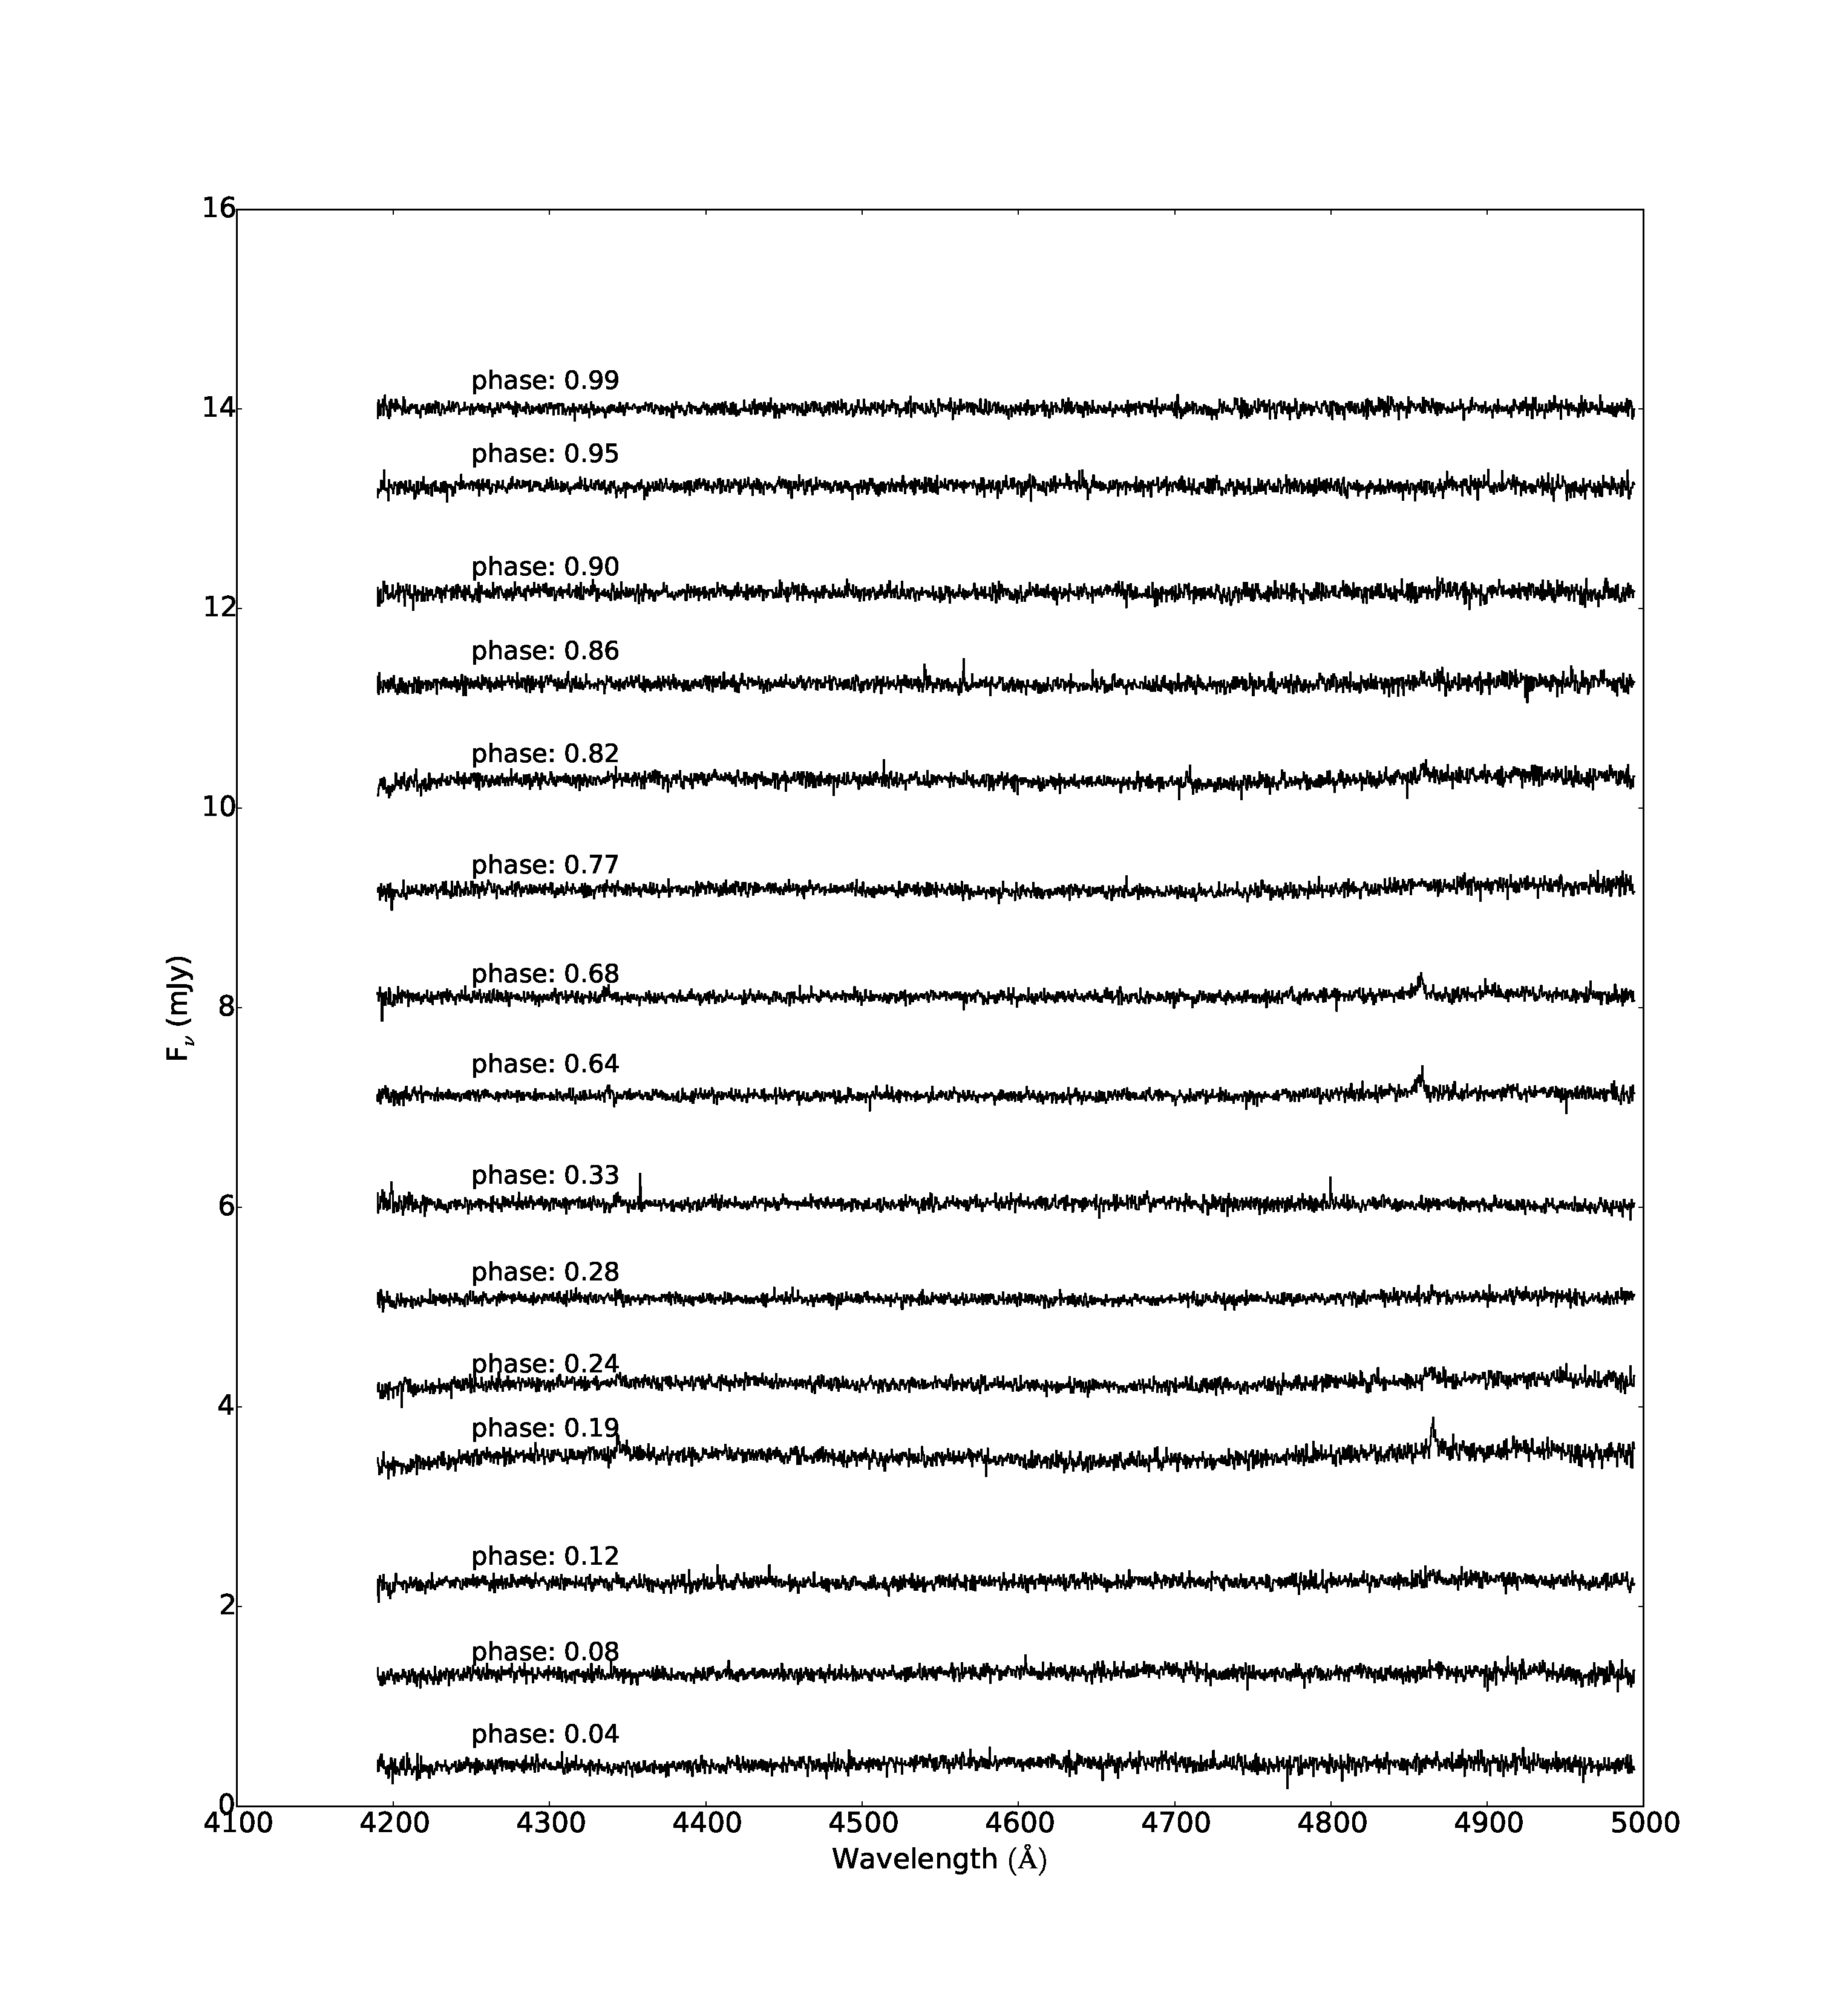
\includegraphics[width=\textwidth]{images/blue_spectra.eps}
\caption[Caption for spectra]{ \emph{This figure to be removed. Only here for reference for the time being.} The blue optical spectra of CRTS\,J0711+4404 taken at 16 stages of the orbital cycle during quiesence in February 2009.  }
\label{fig:spectra-quiescent-blue}
\end{figure*}

\subsection{Radial velocities}
The time resolved spectra taken during quiesence show a clear sodium doublet (Na I) at $8183$~\AA~ and $8194$\AA \, for most of the phases. This feature is associated with the photosphere of the M-dwarf companion. A trail of the spectra shows a clear movement due to doppler shift through the orbital cycle. For each of the 17 spectra we fitted a double gaussian to the spectra using a least squares approach. The gaussian took the form of, 
\begin{equation}f_\lambda = a_0 + a_1 e^{-\frac{1}{2}(\frac{\lambda - a_2}{a_3})^2} + a_4 e^{-\frac{1}{2}(\frac{\lambda - (a_2 - \delta)}{a_3})^2}  \end{equation}
where $f_\lambda$ is the measured flux at the wavelength, $\lambda$. During the least squares convergence we kept the separation $\delta$ fixed at $11 \AA$; the depth of the lines $a_1$ and $a_4$ free to vary but equal to each other and the width of the lines $a_3$ fixed to $3.4 \AA$. The fitted wavelengths were converted to radial velocities and we fitted a sinusoid to the result. The sinusoid's period was fixed to the known orbital period as determined from photometry and quoted in equation~(\ref{eq:ephemeris}). The fitted radial velocity profile is shown in Fig. \ref{fig:rv-fit}. Our fitted radial velocity has a $K_2$ semi-amplitude of $435(12) km.s^{-1}$. 

If we assume a mass of $0.16M_{\odot}$ for the companion star (from \citet{Knigge2011} donor star sequence), with $P_{orb} = 117min$ and using Keplers 3rd law with an inclination $i=90^o$ from \citet{Schwope2015}, this would at imply a $\sim 1M_{\odot}$ white dwarf.

\subsection{Magnetic field strength}
Cyclotron humps are clearly visible in the spectra and especially strong at phases immediately before and after the eclipse. In order to estimate the magnetic field strength we found the wavelength for the hump maxima of two consecutive humps for the spectrum taken at phase 0.12 (as shown in Fig. \ref{fig:spectra-quiescent}) by fitting a quadratic to the continuum. The maxima occured at wavelengths $\lambda  = 8092$ and $6430 \AA$. Using the formula, 
\begin{equation}B = \frac{2 \pi m_e c}{e}(\frac{1}{\lambda_1} - \frac{1}{\lambda_2})\end{equation}
we calculate the field strength at the accretion pole to be $B = 34MG$.

% fit to the Sloane models
\begin{figure*}
\centering
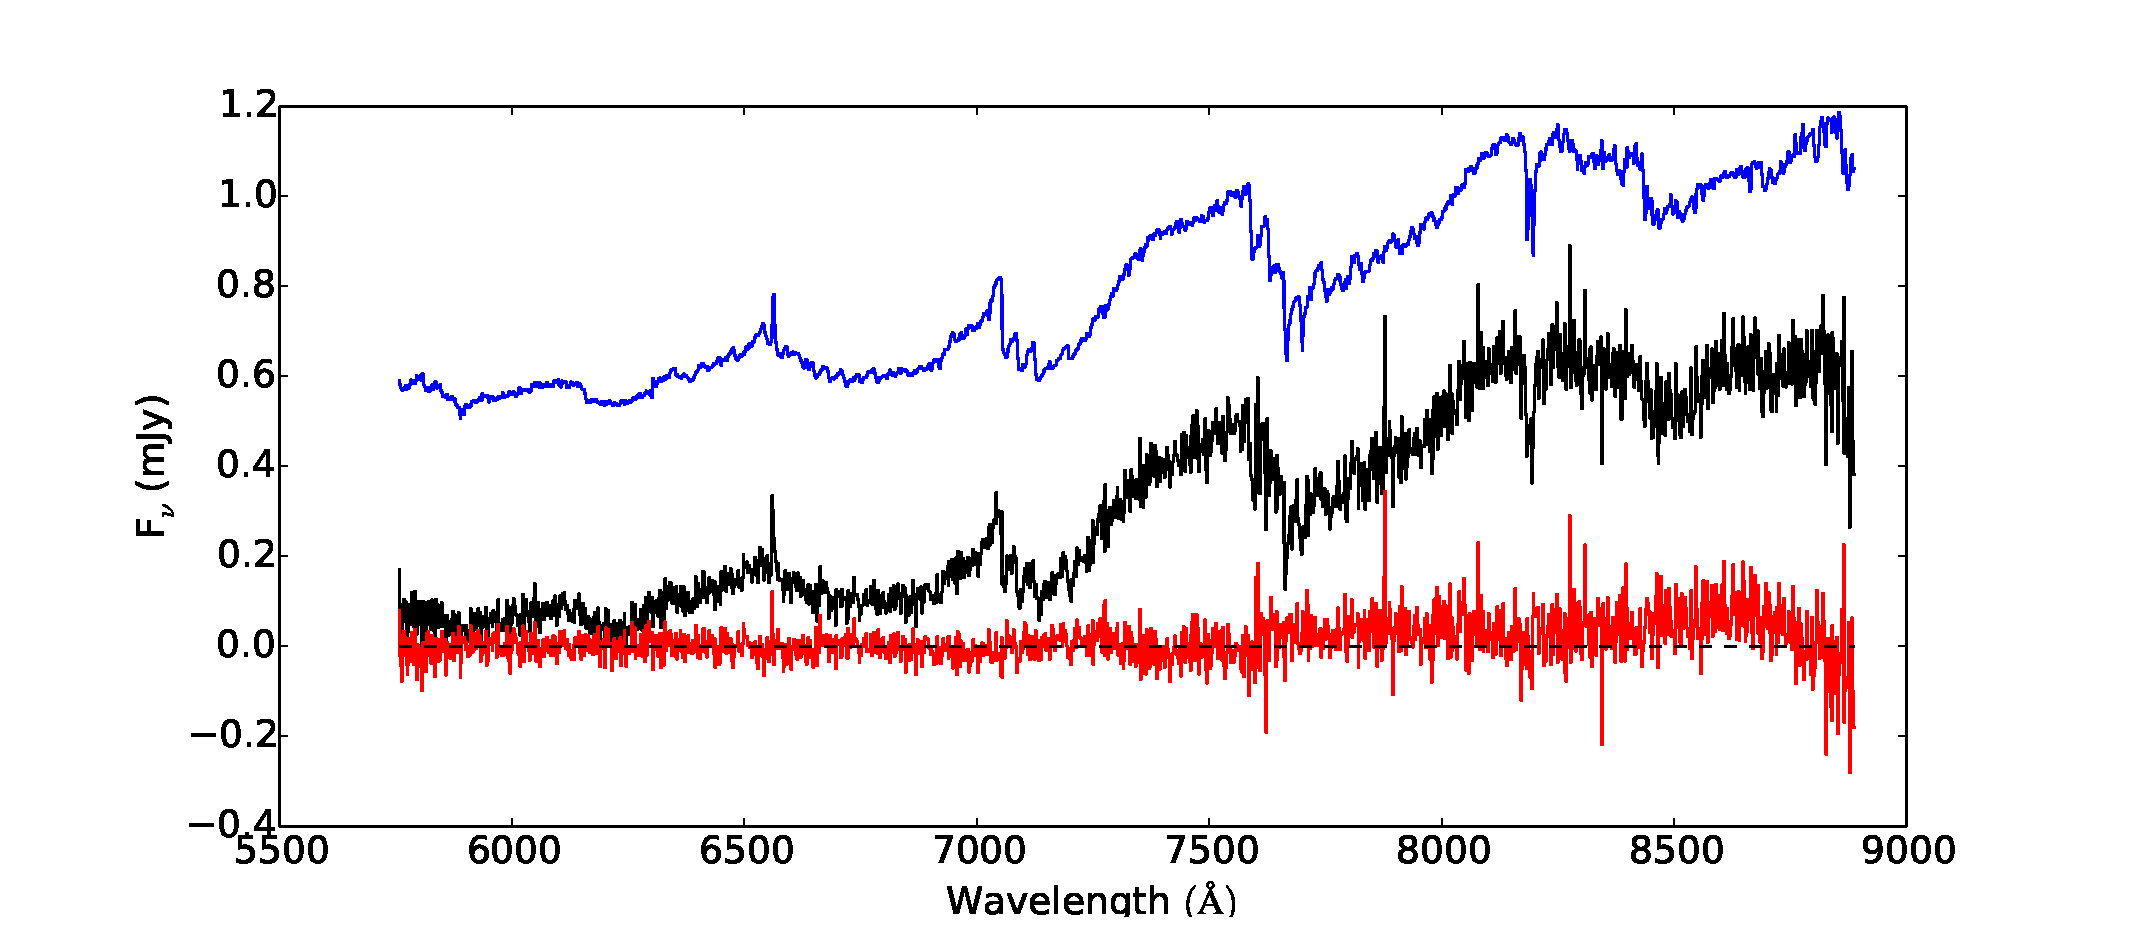
\includegraphics[width=\textwidth]{images/modelfit.eps}
\caption[Caption for spectrum]{The spectrum taken at phase 0.9975 (during primary eclipse) shows the mDwarf secondary without contamination from the accretion stream of the primary. The spectrum was fitted to a list of SDSS template spectra and the best match was to a dM5. Our observed spectrum is in black with the template (offset by 0.5) in blue and our residuals in red. }
\label{fig:sloanfit}
\end{figure*}

% Stacked phased (subtracted spectra)
\begin{figure*}
\centering
\includegraphics[width=\textwidth]{images/subtracted_stacked.eps}
\caption[Caption for spectrum]{The residual spectra, after subtraction of the mDwarf companion.  }
\label{fig:sloanfit}
\end{figure*}


\section{Conclusions}

Conclusions....

\section*{Acknowledgements}
We would like to thank...

%%%%%%%%%%%%%%%%%%%%%%%%%%%%%%%%%%%%%%%%%%%%%%%%%%

%%%%%%%%%%%%%%%%%%%% REFERENCES %%%%%%%%%%%%%%%%%%

% The best way to enter references is to use BibTeX:

\bibliographystyle{mnras}
\bibliography{../rashley} % if your bibtex file is called example.bib


% Alternatively you could enter them by hand, like this:
% This method is tedious and prone to error if you have lots of references
%\begin{thebibliography}{99}
%\bibitem[\protect\citeauthoryear{Author}{2012}]{Author2012}
%Author A.~N., 2013, Journal of Improbable Astronomy, 1, 1
%\bibitem[\protect\citeauthoryear{Others}{2013}]{Others2013}
%Others S., 2012, Journal of Interesting Stuff, 17, 198
%\end{thebibliography}

%%%%%%%%%%%%%%%%%%%%%%%%%%%%%%%%%%%%%%%%%%%%%%%%%%

%%%%%%%%%%%%%%%%% APPENDICES %%%%%%%%%%%%%%%%%%%%%

%\appendix

%\section{Some extra material}

%If you want to present additional material which would interrupt the flow of the main paper,
%it can be placed in an Appendix which appears after the list of references.

%%%%%%%%%%%%%%%%%%%%%%%%%%%%%%%%%%%%%%%%%%%%%%%%%%


% Don't change these lines
\bsp	% typesetting comment
\label{lastpage}
\end{document}

% End of mnras_template.tex